\documentclass{ximera}

%\usepackage{todonotes}

\newcommand{\todo}{}

\usepackage{esint} % for \oiint
\ifxake%%https://math.meta.stackexchange.com/questions/9973/how-do-you-render-a-closed-surface-double-integral
\renewcommand{\oiint}{{\large\bigcirc}\kern-1.56em\iint}
\fi


\graphicspath{
  {./}
  {ximeraTutorial/}
  {basicPhilosophy/}
  {functionsOfSeveralVariables/}
  {normalVectors/}
  {lagrangeMultipliers/}
  {vectorFields/}
  {greensTheorem/}
  {shapeOfThingsToCome/}
  {dotProducts/}
  {partialDerivativesAndTheGradientVector/}
  {../productAndQuotientRules/exercises/}
  {../normalVectors/exercisesParametricPlots/}
  {../continuityOfFunctionsOfSeveralVariables/exercises/}
  {../partialDerivativesAndTheGradientVector/exercises/}
  {../directionalDerivativeAndChainRule/exercises/}
  {../commonCoordinates/exercisesCylindricalCoordinates/}
  {../commonCoordinates/exercisesSphericalCoordinates/}
  {../greensTheorem/exercisesCurlAndLineIntegrals/}
  {../greensTheorem/exercisesDivergenceAndLineIntegrals/}
  {../shapeOfThingsToCome/exercisesDivergenceTheorem/}
  {../greensTheorem/}
  {../shapeOfThingsToCome/}
  {../separableDifferentialEquations/exercises/}
  {vectorFields/}
}

\newcommand{\mooculus}{\textsf{\textbf{MOOC}\textnormal{\textsf{ULUS}}}}

\usepackage{tkz-euclide}
\usepackage{tikz}
\usepackage{tikz-cd}
\usetikzlibrary{arrows}
\tikzset{>=stealth,commutative diagrams/.cd,
  arrow style=tikz,diagrams={>=stealth}} %% cool arrow head
\tikzset{shorten <>/.style={ shorten >=#1, shorten <=#1 } } %% allows shorter vectors

\usetikzlibrary{backgrounds} %% for boxes around graphs
\usetikzlibrary{shapes,positioning}  %% Clouds and stars
\usetikzlibrary{matrix} %% for matrix
\usepgfplotslibrary{polar} %% for polar plots
\usepgfplotslibrary{fillbetween} %% to shade area between curves in TikZ
%\usetkzobj{all}
\usepackage[makeroom]{cancel} %% for strike outs
%\usepackage{mathtools} %% for pretty underbrace % Breaks Ximera
%\usepackage{multicol}
\usepackage{pgffor} %% required for integral for loops



%% http://tex.stackexchange.com/questions/66490/drawing-a-tikz-arc-specifying-the-center
%% Draws beach ball
\tikzset{pics/carc/.style args={#1:#2:#3}{code={\draw[pic actions] (#1:#3) arc(#1:#2:#3);}}}



\usepackage{array}
\setlength{\extrarowheight}{+.1cm}
\newdimen\digitwidth
\settowidth\digitwidth{9}
\def\divrule#1#2{
\noalign{\moveright#1\digitwidth
\vbox{\hrule width#2\digitwidth}}}




% \newcommand{\RR}{\mathbb R}
% \newcommand{\R}{\mathbb R}
% \newcommand{\N}{\mathbb N}
% \newcommand{\Z}{\mathbb Z}

\newcommand{\sagemath}{\textsf{SageMath}}


%\renewcommand{\d}{\,d\!}
%\renewcommand{\d}{\mathop{}\!d}
%\newcommand{\dd}[2][]{\frac{\d #1}{\d #2}}
%\newcommand{\pp}[2][]{\frac{\partial #1}{\partial #2}}
% \renewcommand{\l}{\ell}
%\newcommand{\ddx}{\frac{d}{\d x}}

% \newcommand{\zeroOverZero}{\ensuremath{\boldsymbol{\tfrac{0}{0}}}}
%\newcommand{\inftyOverInfty}{\ensuremath{\boldsymbol{\tfrac{\infty}{\infty}}}}
%\newcommand{\zeroOverInfty}{\ensuremath{\boldsymbol{\tfrac{0}{\infty}}}}
%\newcommand{\zeroTimesInfty}{\ensuremath{\small\boldsymbol{0\cdot \infty}}}
%\newcommand{\inftyMinusInfty}{\ensuremath{\small\boldsymbol{\infty - \infty}}}
%\newcommand{\oneToInfty}{\ensuremath{\boldsymbol{1^\infty}}}
%\newcommand{\zeroToZero}{\ensuremath{\boldsymbol{0^0}}}
%\newcommand{\inftyToZero}{\ensuremath{\boldsymbol{\infty^0}}}



% \newcommand{\numOverZero}{\ensuremath{\boldsymbol{\tfrac{\#}{0}}}}
% \newcommand{\dfn}{\textbf}
% \newcommand{\unit}{\,\mathrm}
% \newcommand{\unit}{\mathop{}\!\mathrm}
% \newcommand{\eval}[1]{\bigg[ #1 \bigg]}
% \newcommand{\seq}[1]{\left( #1 \right)}
% \renewcommand{\epsilon}{\varepsilon}
% \renewcommand{\phi}{\varphi}


% \renewcommand{\iff}{\Leftrightarrow}

% \DeclareMathOperator{\arccot}{arccot}
% \DeclareMathOperator{\arcsec}{arcsec}
% \DeclareMathOperator{\arccsc}{arccsc}
% \DeclareMathOperator{\si}{Si}
% \DeclareMathOperator{\scal}{scal}
% \DeclareMathOperator{\sign}{sign}


%% \newcommand{\tightoverset}[2]{% for arrow vec
%%   \mathop{#2}\limits^{\vbox to -.5ex{\kern-0.75ex\hbox{$#1$}\vss}}}
% \newcommand{\arrowvec}[1]{{\overset{\rightharpoonup}{#1}}}
% \renewcommand{\vec}[1]{\arrowvec{\mathbf{#1}}}
% \renewcommand{\vec}[1]{{\overset{\boldsymbol{\rightharpoonup}}{\mathbf{#1}}}}

% \newcommand{\point}[1]{\left(#1\right)} %this allows \vector{ to be changed to \vector{ with a quick find and replace
% \newcommand{\pt}[1]{\mathbf{#1}} %this allows \vec{ to be changed to \vec{ with a quick find and replace
% \newcommand{\Lim}[2]{\lim_{\point{#1} \to \point{#2}}} %Bart, I changed this to point since I want to use it.  It runs through both of the exercise and exerciseE files in limits section, which is why it was in each document to start with.

% \DeclareMathOperator{\proj}{\mathbf{proj}}
% \newcommand{\veci}{{\boldsymbol{\hat{\imath}}}}
% \newcommand{\vecj}{{\boldsymbol{\hat{\jmath}}}}
% \newcommand{\veck}{{\boldsymbol{\hat{k}}}}
% \newcommand{\vecl}{\vec{\boldsymbol{\l}}}
% \newcommand{\uvec}[1]{\mathbf{\hat{#1}}}
% \newcommand{\utan}{\mathbf{\hat{t}}}
% \newcommand{\unormal}{\mathbf{\hat{n}}}
% \newcommand{\ubinormal}{\mathbf{\hat{b}}}

% \newcommand{\dotp}{\bullet}
% \newcommand{\cross}{\boldsymbol\times}
% \newcommand{\grad}{\boldsymbol\nabla}
% \newcommand{\divergence}{\grad\dotp}
% \newcommand{\curl}{\grad\cross}
%\DeclareMathOperator{\divergence}{divergence}
%\DeclareMathOperator{\curl}[1]{\grad\cross #1}
% \newcommand{\lto}{\mathop{\longrightarrow\,}\limits}

% \renewcommand{\bar}{\overline}

\colorlet{textColor}{black}
\colorlet{background}{white}
\colorlet{penColor}{blue!50!black} % Color of a curve in a plot
\colorlet{penColor2}{red!50!black}% Color of a curve in a plot
\colorlet{penColor3}{red!50!blue} % Color of a curve in a plot
\colorlet{penColor4}{green!50!black} % Color of a curve in a plot
\colorlet{penColor5}{orange!80!black} % Color of a curve in a plot
\colorlet{penColor6}{yellow!70!black} % Color of a curve in a plot
\colorlet{fill1}{penColor!20} % Color of fill in a plot
\colorlet{fill2}{penColor2!20} % Color of fill in a plot
\colorlet{fillp}{fill1} % Color of positive area
\colorlet{filln}{penColor2!20} % Color of negative area
\colorlet{fill3}{penColor3!20} % Fill
\colorlet{fill4}{penColor4!20} % Fill
\colorlet{fill5}{penColor5!20} % Fill
\colorlet{gridColor}{gray!50} % Color of grid in a plot

\newcommand{\surfaceColor}{violet}
\newcommand{\surfaceColorTwo}{redyellow}
\newcommand{\sliceColor}{greenyellow}




\pgfmathdeclarefunction{gauss}{2}{% gives gaussian
  \pgfmathparse{1/(#2*sqrt(2*pi))*exp(-((x-#1)^2)/(2*#2^2))}%
}


%%%%%%%%%%%%%
%% Vectors
%%%%%%%%%%%%%

%% Simple horiz vectors
\renewcommand{\vector}[1]{\left\langle #1\right\rangle}


%% %% Complex Horiz Vectors with angle brackets
%% \makeatletter
%% \renewcommand{\vector}[2][ , ]{\left\langle%
%%   \def\nextitem{\def\nextitem{#1}}%
%%   \@for \el:=#2\do{\nextitem\el}\right\rangle%
%% }
%% \makeatother

%% %% Vertical Vectors
%% \def\vector#1{\begin{bmatrix}\vecListA#1,,\end{bmatrix}}
%% \def\vecListA#1,{\if,#1,\else #1\cr \expandafter \vecListA \fi}

%%%%%%%%%%%%%
%% End of vectors
%%%%%%%%%%%%%

%\newcommand{\fullwidth}{}
%\newcommand{\normalwidth}{}



%% makes a snazzy t-chart for evaluating functions
%\newenvironment{tchart}{\rowcolors{2}{}{background!90!textColor}\array}{\endarray}

%%This is to help with formatting on future title pages.
\newenvironment{sectionOutcomes}{}{}



%% Flowchart stuff
%\tikzstyle{startstop} = [rectangle, rounded corners, minimum width=3cm, minimum height=1cm,text centered, draw=black]
%\tikzstyle{question} = [rectangle, minimum width=3cm, minimum height=1cm, text centered, draw=black]
%\tikzstyle{decision} = [trapezium, trapezium left angle=70, trapezium right angle=110, minimum width=3cm, minimum height=1cm, text centered, draw=black]
%\tikzstyle{question} = [rectangle, rounded corners, minimum width=3cm, minimum height=1cm,text centered, draw=black]
%\tikzstyle{process} = [rectangle, minimum width=3cm, minimum height=1cm, text centered, draw=black]
%\tikzstyle{decision} = [trapezium, trapezium left angle=70, trapezium right angle=110, minimum width=3cm, minimum height=1cm, text centered, draw=black]


\title{Left and Right}

\begin{document}

\begin{abstract}
stretch the domain
\end{abstract}
\maketitle





We have seen that addition (or subtraction) of constants shifts the domain or range and shifts the graph as a rigid object. All of the movement is the same for every point. \\

Multiplication behaves differently.




\subsection*{Stretching Horizontally}







Consider the function $T$ defined as

\[
T(k) = 
\begin{cases}
  -2k-6 & \text{ if }  -8 \leq k < -2 \\
  -k+3 & \text{ if } 0 \leq k < 10
\end{cases}
\]






Graph of $y = T(k)$.





\begin{image}
\begin{tikzpicture}
  \begin{axis}[
            domain=-10:10, ymax=10, xmax=10, ymin=-10, xmin=-10,
            axis lines =center, xlabel=$k$, ylabel=$y$,
            ytick={-10,-8,-6,-4,-2,2,4,6,8,10},
            xtick={-10,-8,-6,-4,-2,2,4,6,8,10},
            ticklabel style={font=\scriptsize},
            every axis y label/.style={at=(current axis.above origin),anchor=south},
            every axis x label/.style={at=(current axis.right of origin),anchor=west},
            axis on top
          ]
          
  \addplot [draw=penColor,very thick,smooth,domain=(-8:-2)] {-2*x-6};
  \addplot [draw=penColor,very thick,smooth,domain=(0:10)] {-x+3};

  \addplot[color=penColor,only marks,mark=*] coordinates{(-8,10)}; 
  \addplot[color=penColor,fill=white,only marks,mark=*] coordinates{(-2,-2)}; 
  \addplot[color=penColor,only marks,mark=*] coordinates{(0,3)}; 
  \addplot[color=penColor,fill=white,only marks,mark=*] coordinates{(10,-7)}; 


    \end{axis}
\end{tikzpicture}
\end{image}




Now, Let's define a new function based on $T$.



Define $W$ by $W(g) = T(2g)$ with the induced domain.



$g$ represents numbers in the the domain of $W$ and $2g$ represents numbers in the domain of $T$.  

The domain of $T$ is $[-8,-2) \cup [0,10)$.


If $2g \in [-8,-2) \cup [0,10)$, then $g \in [-4,-1) \cup [0,5)$

It is like the domain of $T$ is on a rubberband and it shrunk in half. Wherever you are evaluating $W$, you get the value by evaluating $T$ at twice the $W$ domain number.



\begin{example}  Evaluating $W$

\begin{itemize}
\item $W(4) = T\left(\answer{8}\right) = -8+3=-5$
\item $W(-2) = T\left(\answer{-4}\right) = 2$
\item $W\left(\answer{1}\right) = T(2) = 1$
\end{itemize}


\end{example}


The only exception to the stretching idea is $0$.  Since $2 \cdot 0 = 0$, whenever $g = 0$, then $2g = 0$.  While the domain is being stretched, it is being stretched away from $0$. Stretching cannot move $0$. It gets pinned down where it is.


$W(0) = T(0)$.  The rubberband is pinned at $0$, because any multiple of $0$ is still $0$.  

As the functions above demonstrate, multiplication by $2$ compressed the domain.

It seems backwards.  We multiplied by $2$ and the resulting domain was a compressed version of the original domain.  That is because this is a backwards view of what happened, like what we saw with shifting.



We multiplied $g$ by $2$, but $g$ is representing the domain of $W$.  The domain of $W$ is stretching.  We want to know what ``happened'' to the domain of $T$.  $T$ is the old, original function and $k$ represents the domain of $T$.  \\

``What happened to $k$?'' is the question.\\

In our definition of $W$, we have $k=2g$, which gives us $g=\frac{k}{2}$.  \\

$k$ is cut in half, which is what we see in the domain and in the graph and in the formula.  \\

$k$ is replaced with $2g$.




\[
W(g) = 
\begin{cases}
  -2(2g)-6    & \text{ if }  -8 \leq 2g < -2 \\
  -(2g)+3   & \text{ if } 0 \leq 2g < 10
\end{cases}
\]





\[
W(g) = 
\begin{cases}
  -4g-6    & \text{ if }  -4 \leq g < -1 \\
  -2g + 3   & \text{ if } 0 \leq g < 5
\end{cases}
\]








Graph of $z = W(g)$.






\begin{image}
\begin{tikzpicture}
  \begin{axis}[
            domain=-10:10, ymax=10, xmax=10, ymin=-10, xmin=-10,
            axis lines =center, xlabel=$g$, ylabel=$z$,
            ytick={-10,-8,-6,-4,-2,2,4,6,8,10},
            xtick={-10,-8,-6,-4,-2,2,4,6,8,10},
            ticklabel style={font=\scriptsize},
            every axis y label/.style={at=(current axis.above origin),anchor=south},
            every axis x label/.style={at=(current axis.right of origin),anchor=west},
            axis on top
          ]
          
  \addplot [draw=penColor,very thick,smooth,domain=(-8:-1)] {-4*x-6};
  \addplot [draw=penColor,very thick,smooth,domain=(0:5)] {-2*x+3};

  \addplot[color=penColor,only marks,mark=*] coordinates{(-4,10)}; 
  \addplot[color=penColor,fill=white,only marks,mark=*] coordinates{(-1,-2)}; 
  \addplot[color=penColor,only marks,mark=*] coordinates{(0,3)}; 
  \addplot[color=penColor,fill=white,only marks,mark=*] coordinates{(5,-7)}; 


    \end{axis}
\end{tikzpicture}
\end{image}



$T$ and $W$ have the same maximums and minimums.  The height of the points didn't change.  The points to the left of the vertical axis moved to the right. The points to the right of the vertical axis moved to the left as the graph compressed horizontally.




















\subsection*{Negative Coefficients}


What if we mulitply by $-2$ rather than $2$?













Now, Let's define a new function again based on $T$.



Define $M$ by $M(r) = T(-2r)$ with the induced domain.



$r$ represents numbers in the domain of $M$ and now $-2r$ represents numbers in the domain of $T$.  

The domain of $T$ is $[-8,-2) \cup [0,10)$.


If $-2r \in [-8,-2) \cup [0,10)$, then $r \in (-5,0] \cup (1, 4]$








\[
M(r) = 
\begin{cases}
  -2(-2r)-6    & \text{ if }  -8 \leq -2r < -2 \\
  -(-2r)+3   & \text{ if } 0 \leq -2r < 10
\end{cases}
\]





\[
M(r) = 
\begin{cases}
  4r-6    & \text{ if }  1 < r \leq 4 \\
  2r + 3   & \text{ if } -5 < r \leq 0
\end{cases}
\]








It is like the domain of $T$ is on a rubberband and it shrunk in half and then reflected around $0$.  As $r$ walks through the domain of $M$ from left to right, the corresponding walking in the domain of $T$ is from right to left.



\begin{example}  Evaluating $W$

\begin{itemize}
\item $M(4) = T\left(\answer{-8}\right) = 10$
\item $M(-2) = T\left(\answer{4}\right) = -1$
\item $M(\left(\answer{0}\right)) = T(0) = 3$
\end{itemize}


\end{example}


The domain shrinks around $0$. $M(0) = T(0)$.  The rubberband is pinned at $0$, because any multiple of $0$ is still $0$.  









Since this multiplication was on the inside of the function notation, it only affects the domain.  Multiplication by $-1$, reflects the graph across the vertical axis - the domain switches signs. Multiplication by $2$ compresses the graph.



Graph of $m = M(r)$.






\begin{image}
\begin{tikzpicture}
  \begin{axis}[
            domain=-10:10, ymax=10, xmax=10, ymin=-10, xmin=-10,
            axis lines =center, xlabel=$r$, ylabel=$m$,
            ytick={-10,-8,-6,-4,-2,2,4,6,8,10},
            xtick={-10,-8,-6,-4,-2,2,4,6,8,10},
            ticklabel style={font=\scriptsize},
            every axis y label/.style={at=(current axis.above origin),anchor=south},
            every axis x label/.style={at=(current axis.right of origin),anchor=west},
            axis on top
          ]
          
  \addplot [draw=penColor,very thick,smooth,domain=(1:4)] {4*x-6};
  \addplot [draw=penColor,very thick,smooth,domain=(-5:0)] {2*x+3};

  \addplot[color=penColor,only marks,mark=*] coordinates{(4,10)}; 
  \addplot[color=penColor,fill=white,only marks,mark=*] coordinates{(1,-2)}; 
  \addplot[color=penColor,only marks,mark=*] coordinates{(0,3)}; 
  \addplot[color=penColor,fill=white,only marks,mark=*] coordinates{(-5,-7)}; 


    \end{axis}
\end{tikzpicture}
\end{image}


























\begin{example} Sine



Graph of $y = \sin(2\theta)$.

\begin{image}
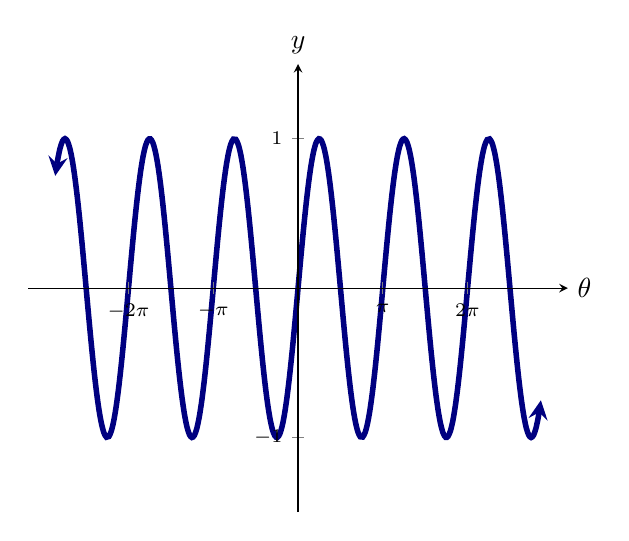
\begin{tikzpicture} 
  \begin{axis}[
            domain=-10:10, ymax=1.5, xmax=10, ymin=-1.5, xmin=-10,
            xtick={-6.28, -3.14, 3.14, 6.28}, 
            xticklabels={$-2\pi$, $-\pi$, $\pi$, $2\pi$},
            axis lines =center,  xlabel={$\theta$}, ylabel=$y$,
            ticklabel style={font=\scriptsize},
            every axis y label/.style={at=(current axis.above origin),anchor=south},
            every axis x label/.style={at=(current axis.right of origin),anchor=west},
            axis on top
          ]
          
          	\addplot [line width=2, penColor, smooth,samples=200,domain=(-9:9), <->] {sin(2*deg(x))};

           

  \end{axis}
\end{tikzpicture}
\end{image}


The graph is compressed horizontally by a factor of $\frac{1}{2}$.


\end{example}




\begin{example} Cosine

Graph of $y = \cos\left(\frac{1}{2}\theta\right)$.

\begin{image}
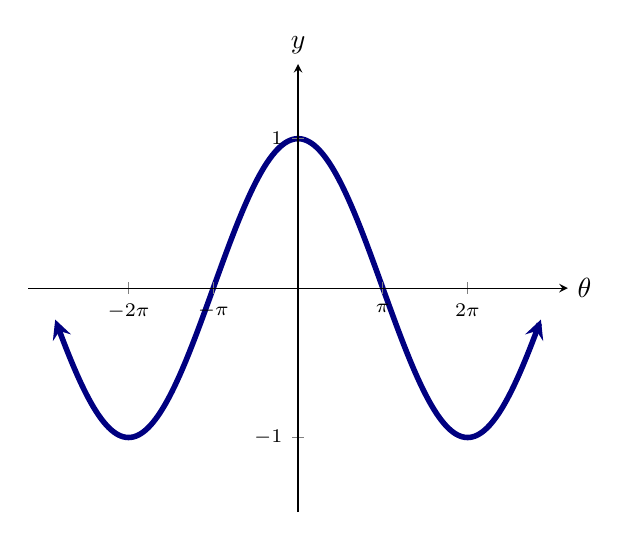
\begin{tikzpicture} 
  \begin{axis}[
            domain=-10:10, ymax=1.5, xmax=10, ymin=-1.5, xmin=-10,
            xtick={-6.28, -3.14, 3.14, 6.28}, 
            xticklabels={$-2\pi$, $-\pi$, $\pi$, $2\pi$},
            axis lines =center,  xlabel={$\theta$}, ylabel=$y$,
            ticklabel style={font=\scriptsize},
            every axis y label/.style={at=(current axis.above origin),anchor=south},
            every axis x label/.style={at=(current axis.right of origin),anchor=west},
            axis on top
          ]
          
          	\addplot [line width=2, penColor, smooth,samples=200,domain=(-9:9), <->] {cos(0.5*deg(x))};

           

  \end{axis}
\end{tikzpicture}
\end{image}


The graph has been stretched horizontally by a factor of $2$.


\end{example}





Multiplication of the domain by a constant doesn't change the shape of the graph.  It might squish it horizontally or stretch it horizontally, but the shape remains.  All of the function characteristics are relatively the same in each graph when you view them from $0$. The maximums and minimums are still in relatively the same places when viewed from $0$.  

You may have to view this in reverse, if the multiplication coefficient was negative, but all of the characteristics and features remain.








\begin{example} Absolute Value



Graph of $y = |3r|$.



\begin{image}
\begin{tikzpicture} 
  \begin{axis}[
            domain=-10:10, ymax=10, xmax=10, ymin=-10, xmin=-10,
            axis lines =center, xlabel=$r$, ylabel=$y$,
            ytick={-10,-8,-6,-4,-2,2,4,6,8,10},
            xtick={-10,-8,-6,-4,-2,2,4,6,8,10},
            ticklabel style={font=\scriptsize},
            every axis y label/.style={at=(current axis.above origin),anchor=south},
            every axis x label/.style={at=(current axis.right of origin),anchor=west},
            axis on top
          ]
          
          \addplot [line width=2, penColor, smooth, samples=200, domain=(-3:3),<->] {3*abs(x)};
        

  \end{axis}
\end{tikzpicture}
\end{image}



Multiplication by $3$ compresses the graph, because all domain numbers here correspond to $3$ times their values in the domain of $|x|$, therefore the graph is steeper.






\end{example}







\begin{example}

Here is the graph of $y = \log_2(-t)$.




\begin{image}
\begin{tikzpicture} 
  \begin{axis}[
            domain=-10:10, ymax=10, xmax=10, ymin=-10, xmin=-10,
            axis lines =center, xlabel=$t$, ylabel=$y$,
            ytick={-10,-8,-6,-4,-2,2,4,6,8,10},
            xtick={-10,-8,-6,-4,-2,2,4,6,8,10},
            ticklabel style={font=\scriptsize},
            every axis y label/.style={at=(current axis.above origin),anchor=south},
            every axis x label/.style={at=(current axis.right of origin),anchor=west},
            axis on top
          ]
          
          \addplot [line width=2, penColor, smooth,samples=200,domain=(-8.1:-0.07),<->] {ln(-x)/ln(2)};
          \addplot [line width=1, gray, dashed,domain=(-9:9),<->] ({0},{x});

          \addplot[color=penColor,only marks,mark=*] coordinates{(-1,0)}; 

           

  \end{axis}
\end{tikzpicture}
\end{image}


The graph looks the same as the basic logarithm graph, just reflected about the vertical axis.




\end{example}









\begin{example} Stretching Domains

Compared to the graph of the function $y=f(x)$, the graph of $z=g(r)=f(4r)$ looks to be 

\begin{multipleChoice}

\choice{shifted left by $4$}
\choice{shifted right by $4$}
\choice{stretched by a factor of $4$}
\choice[correct]{compressed by a factor of $\frac{1}{4}$}
\end{multipleChoice}


\end{example}





















\begin{center}
\textbf{\textcolor{green!50!black}{ooooo-=-=-=-ooOoo-=-=-=-ooooo}} \\

more examples can be found by following this link\\ \link[More Examples of Stretching]{https://ximera.osu.edu/csccmathematics/precalculus1/precalculus1/stretching/examples/exampleList}

\end{center}







\end{document}
